\documentclass[a4paper]{jpconf}
%\bibliographystyle{iopart-num}
%\usepackage{citesort}
\usepackage{graphicx}

\begin{document}
\title{A Geant4 physics list for spallation and related nuclear physics applications 
based on INCL and ABLA models}

\author{A Heikkinen$^1$, A Boudard$^2$, P Kaitaniemi$^2$ and G Folger$^3$}

%\author{P J Smith$^1$, T M Collins$^2$, 
%R J Jones$^{3,}$\footnote[4]{Present address:
%Department of Physics, University of Bristol, Tyndalls Park Road, 
%Bristol BS8 1TS, UK.} and Janet Williams$^3$}

\address{$^1$ Helsinki Institute of Physics, P.O. Box 64, FIN-00014 University of Helsinki, Finland}
\address{$^2$ CEN-Saclay, CEA-IRFU/SPhN, 91 191 Gif sur Yvette, France}
\address{$^3$ European Organization for Nuclear Research (CERN), Switzerland}

\ead{aatos.heikkinen@cern.ch}

\begin{abstract}
We present a new Geant4 physics list prepared for nuclear physics applications
in the domain dominated by spallation.
We discuss new Geant4 physics of the C++ translation of original Fortran 
INCL intra-nuclear cascade and ABLA fission/de-excitation codes.
that are used in the physic list.
The INCL model is well established for targets heavier than Aluminium
and projectile energies from $\sim$ 150 MeV up to 2.5 GeV $\sim$ 3 GeV.
Validity of the Geant4 physics list is demonstrated from the perspective of accelerator driven systems
and EURISOL project, especially with the neutron double differential cross sections and residual
nuclei production.
Foreseen improvements of the physics models for the treatment of light targets (Carbon - Oxygen)
and light ion beams (up to Carbon) are discussed.
An example application utilizing the physics list is introduced.
\end{abstract}

\section{Introduction}
 



\begin{figure}[h]
%\begin{minipage}{14pc}

\begin{center}
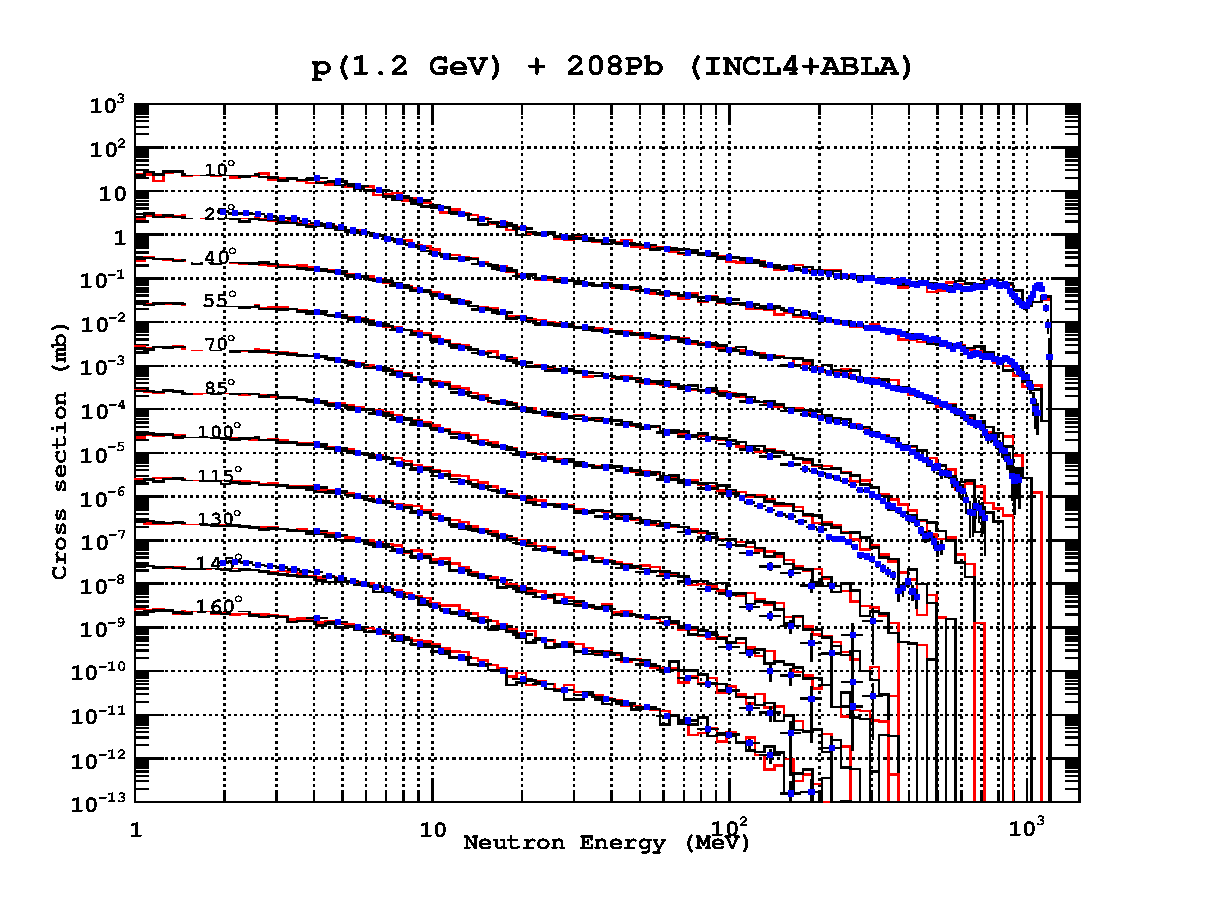
\includegraphics[width=30pc]{poster/images/lead.eps}
\end{center}
\caption{\label{label}Figure caption .}
%\end{minipage}\hspace{2pc}%
%\begin{minipage}{14pc}
%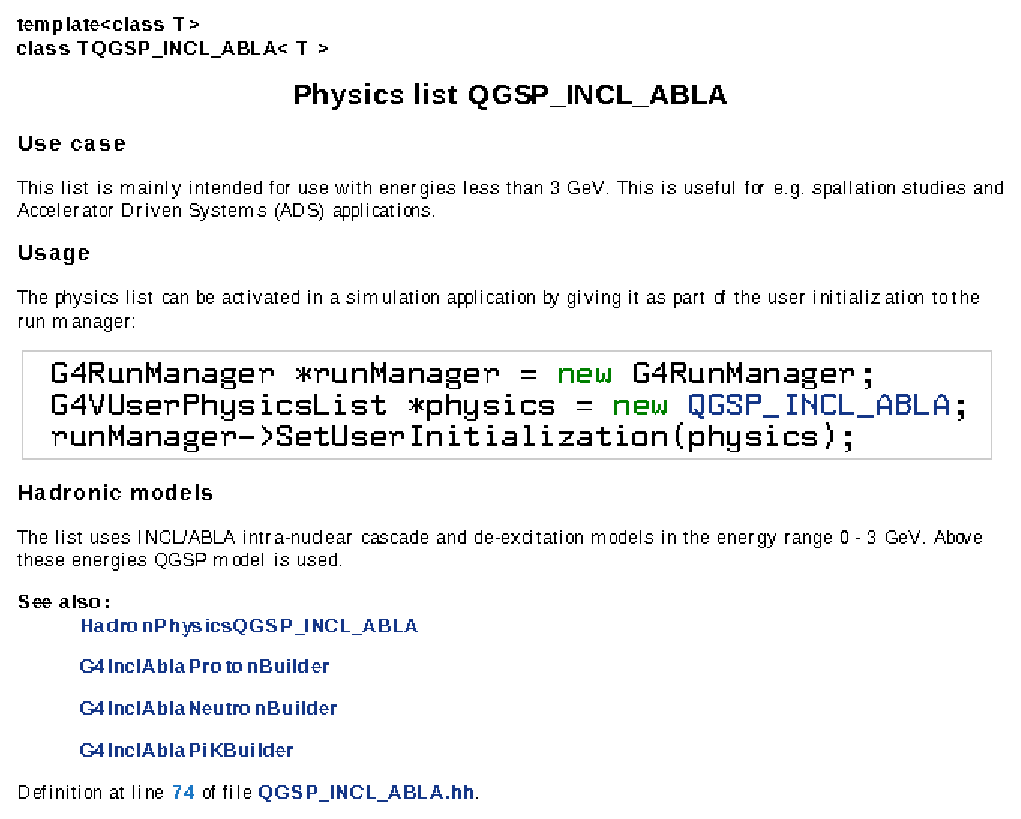
\includegraphics[width=14pc]{./poster/images/inclAblaDoc.eps}
%\caption{\label{label}Figure caption for second of two sided figures.}
%\end{minipage} 
\end{figure}

\begin{figure}[h]
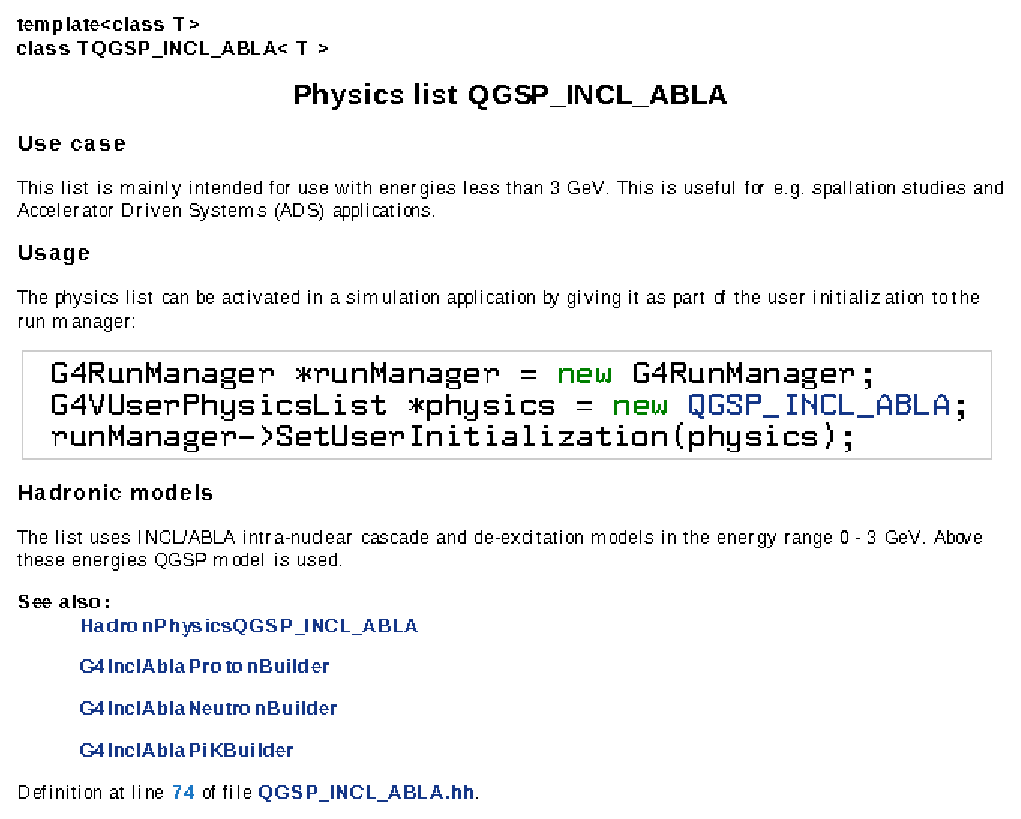
\includegraphics[width=21pc]{poster/images/inclAblaDoc.eps}\hspace{2pc}%
\begin{minipage}[b]{14pc}\caption{\label{label}Figure caption for a narrow figure where the caption is put at the side of the figure.}
\end{minipage}
\end{figure}


\ack %command \ack sets the acknowledgments heading as an unnumbered section.


\appendix % The command \appendix" is used to signify the start of the appendixes.
\section{AH:::}

%\begin{equation}
%time= money
%\end{equation}

%To obtain a simple heading of `Appendix' use the code \verb"\section*{Appendix}". 
%If it contains numbered equations, figures or tables the command \verb"\appendix" should
%precede it and \verb"\setcounter{section}{1}" must follow it. 


\section*{References}



Ref. [1]

\begin{thebibliography}{9}
\item Strite S and Morkoc H 1992 {\it J. Vac. Sci. Technol.} B {\bf 10} 1237 
\item Jain S C, Willander M, Narayan J and van Overstraeten R 2000 
{\it J. Appl. Phys}. {\bf 87} 965 
\end{thebibliography}


\end{document}


